\documentclass[10pt,a4paper]{article}
\usepackage[utf8]{inputenc}
\usepackage[catalan]{babel}
\usepackage{amsmath}
\usepackage{amsfonts}
\usepackage{amssymb}
\usepackage{graphicx}
\usepackage{setspace}
\usepackage{parskip}
\usepackage{amsthm}
\usepackage{fancyhdr}
\usepackage{booktabs}
\usepackage{hyperref}
\usepackage{pgfplots}% This uses tikz
\pgfplotsset{compat=newest}% use newest version
\usepackage{sidecap}
\usepackage{tikz}
\usepackage{tikz-3dplot}
\usepackage{xcolor}
\usepackage{xstring}
\usepackage{circuitikz}
\usepackage{caption}
\usepackage{listings}
\usepackage{array,amsfonts}
\usepackage{setspace}
\captionsetup{justification=centering}
\usetikzlibrary{plotmarks}
\usepackage[left=2.2cm,right=2.2cm,top=3cm,bottom=2.5cm]{geometry}

% Definició de colors
\definecolor{blue2}{HTML}{206B99}
\hypersetup{colorlinks=true, linkcolor=blue2}

% Commandes útils
\DeclareMathOperator{\nim}{nim}
\newcommand{\hs}{\hspace{3pt}}
\newcommand{\sii}{\hspace{3pt} \Leftrightarrow \hspace{3pt}}
\newcommand{\implica}{\hspace{3pt} \Rightarrow \hspace{3pt}}
\newcommand\myfunc[5]{%
  \begingroup
  \setlength\arraycolsep{0pt}
  #1\colon\begin{array}[t]{c >{{}}c<{{}} l}
             #2 & \to & #3 \\ #4 & \mapsto & #5 
          \end{array}%
  \endgroup}

% Vectors i matrius
\newcommand{\mb}{\left( \begin{matrix}}
\newcommand{\me}{\end{matrix} \right)}

% Títol i subtítol
\newcommand{\Title}[1]{\begin{center}\begin{LARGE}#1\vspace{8pt}\end{LARGE}\end{center}}
\newcommand{\SubTitle}[1]{\begin{center}#1\vspace{20pt}\end{center}}

% Espaiat entre línies
\doublespacing

% Inserció de codis
\definecolor{mGreen}{rgb}{0,0.6,0}
\definecolor{mGray}{rgb}{0.5,0.5,0.5}
\definecolor{mPurple}{rgb}{0.58,0,0.82}
\definecolor{backgroundColour}{rgb}{0.95,0.95,0.92}

\definecolor{codegreen}{rgb}{0,0.6,0}
\definecolor{codegray}{rgb}{0.5,0.5,0.5}
\definecolor{codepurple}{rgb}{0.58,0,0.82}
\definecolor{backcolour}{rgb}{0.95,0.95,0.92}

\definecolor{mGreen}{rgb}{0,0.6,0}
\definecolor{mGray}{rgb}{0.5,0.5,0.5}
\definecolor{mPurple}{rgb}{0.58,0,0.82}
\definecolor{backgroundColour}{rgb}{0.95,0.95,0.92}

\lstdefinestyle{CStyle}{
    backgroundcolor=\color{backgroundColour},   
    commentstyle=\color{mGreen},
    keywordstyle=\color{magenta},
    numberstyle=\tiny\color{mGray},
    stringstyle=\color{mPurple},
    basicstyle=\footnotesize,
    breakatwhitespace=false,         
    breaklines=true,                 
    captionpos=b,                    
    keepspaces=true,                 
    numbers=left,                    
    numbersep=5pt,                  
    showspaces=false,                
    showstringspaces=false,
    showtabs=false,                  
    tabsize=2,
    language=C,
    frame=single
}


\lstset{style=CStyle}

% Capçalera a pàgines 2...*
\pagestyle{fancy}
\fancyhf{}
\rhead{Dennis Lucas Buchholz}
\lhead{Implementation eines Textgenerators auf Basis eines Markovprozesses}
\cfoot{\thepage}
\thispagestyle{plain}
\begin{document}
\begin{spacing}{1}

\Title{Implementation eines Textgenerators auf Basis eines Markovprozesses}
\texttt{Autor}: Dennis Lucas Buchholz


\section{Einleitung}

In dieser Dokumentation wird die Implementation eienr Aufgabe in der
Programmiersprache C beschrieben. Ziel dieser Aufgabe ist es, ein Programm zu
erstellen, welches eine Datei einliest und ein stochastisches Markov-Model für den
Inhalt dieser Datei generiert. Auf Basis dieses stochasitsichen Modells 
wird anschließend ein neuer Text ausgegeben. 

Zur Kompilierung und Testen des Quelltextes wurde der Kompilierer
\textbf{gcc} in der Version 9.2.0, GNU \textbf{make} in der Version 3.82.90
und GNU \textbf{ld} (binutils 2.32) aus MinGW verwendet.
Für die Erstellung der Dokumentation wurde \textbf{texify} von MiKTeX 22.8.28
verwendet.

Hinweis: Für die Erstellung dieses Quelltextes wurde die Bibliothek
\textbf{utest.h} für Unit-Tests benutzt. Die Erstellung von Unit-Tests stellt
keinen Anteil an der Aufgabe dar, jedoch haben die Unit-Tests zur Fehlebehebung
und Testung einzelner Programmabschnitte beigetragen. In der Dokumentation wird
auf die Unit-Tests nicht weiter eingegangen.

\subsection{Verzeichnisstruktur}

\begin{tabular}{ l l }
\texttt{/doc} & Alle Dokumentationsdateien \\
\texttt{/include} & Alle Headerdateien (*.h) \\
\texttt{/src} & Alle Quellcodedateien (*.c) \\
\texttt{/test} & Alle Unit-Tests (*.c, *.h) \\
\end{tabular}

\subsection{Make Befehle}
\begin{tabular}{ l l }
    \texttt{make} & Alles (Kompiliere Programm und erstelle Dokumentation) \\
    \texttt{make shakespeare} & Kompiliere Programm \\
    \texttt{make test} & Kompiliere die Unit-Tests und führe sie aus \\
    \texttt{make clean} & Alle Objektdateien aufräumen \\
\end{tabular}

\subsection{Angeforderte Parameter}
\begin{tabular}{ l l }
    \texttt{-h} & Gebe die Hilfeseite aus \\
    \texttt{-f <file>} & Lese die Datei ein \\
    \texttt{-s <n>} & Länge des Suchstrings (standardmäßig: 1 ) \\
    \texttt{-l <n>} & Länge der Ausgabe (standardmäßig: Dateigröße in Bytes) \\
\end{tabular}

\section{Allgemeine Struktur des Programms}
\subsection{Erkennen der Parameter}

Zu Beginn des Programms gilt es zu erkennen, welche Parameter übergeben wurden.
Hierfür wird die Funktion \texttt{parse\_arguments} verwendet, welche mit Hilfe
der \texttt{getopt} Funktion aus der Bibliothek unistd.h alle Parameter
auswertet.

\begin{lstlisting}
FILE* file = stdin;
char* file_name = malloc(sizeof(char) * 256);
file_name[0] = '\0';
size_t input_length, output_length;

parse_arguments(argc, argv, file_name, &input_length, &output_length);
\end{lstlisting}

An \texttt{parse\_arguments()} werden die Anzahl der Argumente und ein
Array mit den Argumenten übergeben. Des Weiteren werden Zeiger auf den
Dateinamen, auf die Suchstringlänge und auf die Ausgabelänge übergeben.
Auf den Adressen dieser Zeiger sollen die jeweiligen Werte gespeichert werden.

In der Funktion \texttt{parse\_arguments()} werden mit Hilfe von
\texttt{sscanf()} die numerischen Argumente (Suchstringlänge \& Ausgabelänge)
eingelesen und versucht in einen unsignierten Integer zu konvertieren.
Sollte die Konvertierung fehlschlagen, so soll sich das Programm beenden und eine
Fehlermeldung ausgeben. Wenn ein Dateiname übergeben wurde soll außerdem überprüft werden, ob sich diese
Datei öffnen lässt. Ist dies der Fall, wird der Dateiname an dem
Speicherort des Zeigers {\it file\_name \/} gespeichert. Sollte dies nicht der
Fall sein, wird sich das Programm beenden und eine Fehlermeldung ausgeben.

\section{Einlesen in einen binären Suchbaum}

\subsection{Einleitung}
Als Datenstruktur für die Speicherung von Suchstrings wurde ein binärer Suchbaum
gewählt. Ein Vorteil eines binäreren Suchbaums ist es, dass die Speicherung
und Abfrage der Suchstrings immer den gleichen Regeln unterliegt.  
Es könnte als Beispiel davon ausgegangen werden, dass ein binärer Suchbaum
mit dem Wurzelknoten ("Basel") vorliegt. Ist der in den Funktionsparametern
angegebene Suchstring (z.B. "Aargau") lexikalisch kleiner als der String des
aktuellen Knotens, so wird dieser als linker Unterknoten eingefügt.
Ist der angegebene Suchstring  (z.B. "Zürich") lexikalisch größer als der String
des aktuellen Knotens, so wird dieser als rechter Unterknoten eingefügt.
Ist der angegebene Suchstring lexikalisch identisch mit dem String des
Wurzelknotens, so muss kein neuer Knoten angelegt werden.

\subsection{Speichern von Zuständen eines Suchstrings}
Um einen zufälligen Text zu erzeugen, wird der initiale Suchstring modifiziert.
Bei jeder Iteration werden alle Zeichen des aktuellen Suchstrings um ein
Zeichen nach links verschoben. Somit fällt das erste Zeichen weg,
und an die letzte Stelle des Suchstrings wird das nächste Zeichen in der Datei
gesetzt. Wenn als Beispiel der Inhalt einer Datei ``Hello World''ist, dann sieht
bei einer Suchstringlänge von 5 sieht der Verlauf der Zustände dieses
Suchstrings so aus:\newline
 \texttt{``Hello''} \textrightarrow \texttt{``ello ''} \textrightarrow \texttt{``llo W''}
\textrightarrow \texttt{``lo Wo''} \textrightarrow \texttt{``o Wor''} \textrightarrow
\texttt{`` Worl''} \textrightarrow \texttt{``World''}

Dieses Verfahren wird im Programm nun mit einer Suchstringlänge {\it n\/} mit den Zeichen einer
ganzen Datei durchgeführt. Hierzu wird eine Datei in \texttt{tree\_from\_file()}
Zeichen für Zeichen ausgelesen und jeder Zustand dieses Suchstrings wird mit Hilfe
der Funktion \texttt{node\_insert()} innerhalb eines neuen Knotens in dem binären
Suchbaum gespeichert. Ebenso wird bei jeder Iteration der Buchstabe in dem
Knoten gespeichert, welcher auf den Suchstring folgt. Wenn ein Suchstring also
mehrfach im Text vorkommt, so wird sich jeder dieser Folgebuchstaben in
dem dazugehörigen Knoten gemerkt.

Durch das Speichern der Folgebuchstaben eines
Suchstrings kann im weiteren Verlauf mit Hilfe eines Markovprozesses
vorausgesagt werden, welcher Zustand des Suchstrings am wahrscheinlichsten
folgen könnte.

\section{Berechnung des Markovmodells}

\subsection{Einleitung}

\begin{align}
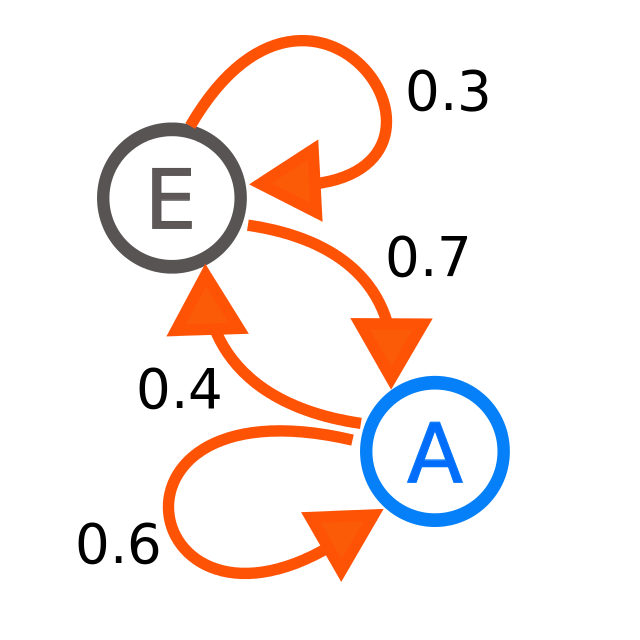
\includegraphics[width=3cm]{markov1.png}
\end{align}

Bei einem Markov-Prozess handelt es sich um einen stochastischen Prozess.
Es liegt ein System vor, für das es zu bestimmten Zeitpunkten Zustände
gibt und ein Ergebnis, welches immer einen zufällig gewählten Zustand darstellt.
Dieser Markov-Prozess enthält Zufallsvariablen, die in Abhängigkeit von bestimmten
Annahmen und eindeutigen Wahrscheinlichkeitsregeln von einem Zustand in einen
anderen übergehen. Der nächste Übergang in einen anderen Zustand hängt nur von
dem vorherigen Zustand und nicht von der Abfogle der Zustände ab.
Diese Annahme erleichtert die Berechnung der bestimmten Wahrscheinlichkeit:

\begin{align}
\text{P}_{i, j} = P(X_{m+1} = j|X_{m} = i)
\end{align}

\subsection{Datenstrukturen für das Markovmodell}

Als Datenstruktur für das Markovmodell wird eine Struktur mit der Bezeichnung
{\it MarkovModel\/} verwendet. Die Struktur enthält einen Zeiger auf die
Speicheradresse von dem Suchstring, die Suchstringlänge, die Ausgabelänge und
einen Zeiger auf die Speicheradresse des binären Suchbaums mit allen möglichen
Zuständen des Suchstrings: 

\begin{lstlisting}
typedef struct MarkovModel MarkovModel;
struct MarkovModel {
    char* search_string;
    size_t search_length;
    size_t output_length;
    Tree* tree;
};
\end{lstlisting}

Die Datenstruktur des binären Suchbaums ist eine Struktur mit der Bezeichnung
{\it Tree\/}, welche lediglich einen Zeiger auf den Wurzelknoten des Baumes
und die Summe aller Knoten beinhaltet. Die Datenstruktur eines einzigen Knotens
ist eine Struktur mit der Bezeichnung {\it Node\/}, die beinhaltet einen Zeiger
auf die Speicheradresse ihres Inhalts, Zeiger auf den linken und rechten
Unterknoten, die Länge ihres Inhalts und einen Zeiger auf eine verkettete Liste
mit möglichen Folgebuchstaben.

\begin{lstlisting}
typedef struct Node Node;
typedef struct Tree Tree;

struct Node {
    char* content;
    Node* left;
    Node* right;
    size_t length;
    List* list_char;
};

struct Tree {
    Node* root;
    size_t node_len;
};
\end{lstlisting}

Als Dateistruktur für die Wahrscheinlichkeiten des Markovprozesses wurde eine
verkettete Liste verwendet. Für jeden möglichen Folgebuchstaben auf einen Suchstring wird ein
Knoten in dieser verketten Liste erstellt. Die Strukturen der verketteten Liste
und dessen Knoten sind folgendermaßen deklariert:
\begin{lstlisting}
typedef struct ListNode ListNode;
typedef struct List List;

struct ListNode {
    char character;
    int frequency;
    double probability;
    ListNode* next_element;
};

struct List {
    ListNode* head;
    int sum_of_frequencies;
};
\end{lstlisting}
In einem Knoten der verketteten Liste wird das Zeichen, die Häufigkeit dieses
Zeichens, die Wahrscheinlichkeit dieses Zeichens und ein Zeiger auf den nächsten
Knoten erfasst. In der Struktur der Liste wird nur ein Zeiger auf den
Kopfknoten und die Summe der Häufigkeiten aller Zeichen erfassen.

Konkret wird die Wahrscheinlichkeit für ein Zeichen folgendermaßen berechnet:
\begin{lstlisting}
void calculate_probabilities(Node* root) {
    ListNode* list_node = root->list_char->head;

    while (list_node != NULL) {
        list_node->probability = (double) list_node->frequency /
                                    root->list_char->sum_of_frequencies;
        list_node = list_node->next_element;
    }

    if(root->left)
        calculate_probabilities(root->left);
    if(root->right)
        calculate_probabilities(root->right);
}
\end{lstlisting}

Alle Knoten des binären Suchbaums werden im Preorder-Verfahren traversiert,
dabei wird für jeden Knoten die verkettete Liste mit den Folgebuchstaben
iteriert. Für jeden Knoten in der Liste wird nun die Wahrscheinlichkeit
berechnet, indem die Häufigkeit dieses Buchstabens nach diesem Suchstrings durch
die Summe der Häufigkeit aller auftretenden Folgebuchstaben dividiert wird.

\subsection{Zufällige Auswahl von Knoten mit Wahrscheinlichkeitsverteilung}

Auf Basis der Wahrscheinlichkeitswerte jedes Knotens in den verketteten Liste 
im binären Suchbaum kann nun vorausgesagt werden, welcher Folgebuchstabe am
wahrscheinlichsten ist. Diese Zufallsentscheidung ist folgendermaßen
implementiert:
\begin{lstlisting}
ListNode* weighted_random(ListNode* head) {
    double s = rand() / (RAND_MAX + 1.0);
    ListNode* list_node = head;
    while (list_node->next_element != NULL
            && ((s -= list_node->probability) >= 0))
        list_node = list_node->next_element;

    return list_node;
}
\end{lstlisting}
Es wird eine Variable mit einem Zufallswert zwischen 0.0 und 1.0 deklariert,
von welcher bei jeder Iteration die Wahrscheinlichkeit eines Knotens der Liste
subtrahiert wird. Sobald der Wert dieser Variable kleiner oder gleich 0 beträgt,
wird der Knoten ausgewählt, von welchem die Wahrscheinlichkeit zuletzt
subtrahiert wurde. Auf diese Weise wurde nun ein Knoten mit einem Folgebuchstaben
 zufällig, aber auf Basis seiner Wahrscheinlichkeit gewählt.

\pagebreak

\subsection{Textausgabe auf Basis einer Wahrscheinlichkeitsverteilung}

Auf Basis der Wahrscheinlichkeitsverteilung kann nun ein neuer Text erstellt
werden. Zunächst wird der initiale Suchstring ausgegeben, welcher sich aus den
ersten Buchstaben der Eingabedatei mit der Suchstringlänge {\it n\/} zusammensetzt.
Daraufhin wird ein Knoten mit dem Inhalt des Suchstrings in dem binären Suchbaum
mit der Funktion \texttt{lookup()} gesucht,
wird ein solcher Knoten gefunden, so wird ein zufälliger aber wahrscheinlicher Buchstabe
mit Hilfe von \texttt{weighted\_random()} gewählt und asugegeben.

Ebenso werden
alle Zeichen des Suchstrings um eine Position nach links verschoben und
der gewählte Buchstabe wird an den Suchstring angehangen. Dieser Prozess wird
wiederholt, sobald genau so viele Zeichen ausgegeben wurden, wie mit der
Ausgabelänge {\it m\/} angegeben. Konkret wurde dies folgendermaßen implementiert:

\begin{lstlisting}
char next_letter(MarkovModel *state) {
    Node* n = lookup(state->tree->root, state->search_string,
                        state->search_length);
    if(!n) {
        model_destroy(state);
        fprintf(stderr,
                "Error: Unable to make prediction for search string '%s'",
                state->search_string);
        exit(EXIT_FAILURE);
    }
    return weighted_random(n->list_char->head)->character;
}
void generate_text(MarkovModel *model) {
    char last_letter;
    srand((unsigned int) time(NULL));

    printf("<%s>", model->search_string);

    for (int i = 0; i < (int) model->output_length; i++) {
        last_letter = next_letter(model);
        printf("%c", last_letter);
        shift_string(model->search_string, (int) model->search_length);
        model->search_string[model->search_length - 1] = last_letter;
    }
}
\end{lstlisting}

Wenn die Beispieldatei ``7zara10.txt'' aus der Aufgabe eingelesen wird, kann die
zufällige Textausgabe des Programms demonstriert werden:
\begin{lstlisting}
$ ./shakespeare -s 19 -l 600 -f 7zara10.txt
<Friedrich Nietzsche>

Also sprach Zarathustra. Der Heilige antwortete: Ich mache Lieder und singe sie,
 und wenn ich Lieder mache, lache, weine und brumme ich: also lobe ich Gott.
Mit Singen, Weinen, Lachen und Brummen lobe ich den Gott, der mein Gott ist.
Doch was bringst du uns zum Geschenke?
Als Zarathustra diese Reden sprach, stand er nahe dem Eingange seiner Hoehle lag.
Aber, indem er mit den Haenden um sich und ueber sich und unter sich griff, und
den zaertlichen Voegeln wehrte, 
siehe, da geschah ihm etwas noch Seltsameres: er griff naemlich dabei unvermerkt
 in ein dichtes warmes Haar-Gezottel hinein;
\end{lstlisting}

Bei erneutem Einlesen ist eine andere Ausgabe ersichtlich:
\begin{lstlisting}
$ ./shakespeare -s 19 -l 600 -f 7zara10.txt
<Friedrich Nietzsche>

Also sprach Zarathustra. Zwar ihr sagt: "die Lust an kleinen Bosheiten erspart
 uns manche grosse boese That." Aber hier sollte man nicht sparen wollen.
 Wie ein Geschwuer ist die boese That: sie juckt und kratzt und bricht heraus,
 - sie redet ehrlich. "Siehe, ich bin Krankheit" - so redet die boese That;
 das ist ihre Ehrlichkeit. 
Aber dem Pilze gleich ist der kleine Gedanke: er kriecht und duckt
\end{lstlisting}


\end{spacing}
\end{document}